
\vspace{-0.3cm}
\begin{IEEEbiography}[{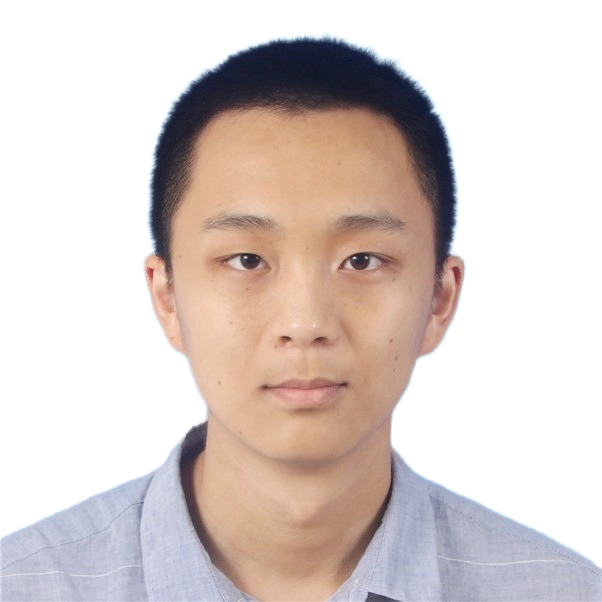
\includegraphics[width=1in,height=1.25in,clip,keepaspectratio]{images/photo/hong.png}}]{Yuncong Hong}
    received his B.ENG degree in electrical and electronic engineering from Southern University of Science and Technology of China (SUSTech) in 2018. He is currently in a joint Ph.D program in computer science with the University of Hong Kong (HKU) and SUSTech. He is co-supervised by Prof. Francis Lau and Prof. Rui Wang. His research interests include edge computing, approximation MDP and online learning.
\end{IEEEbiography}
\vspace{-1cm}

\begin{IEEEbiography}[{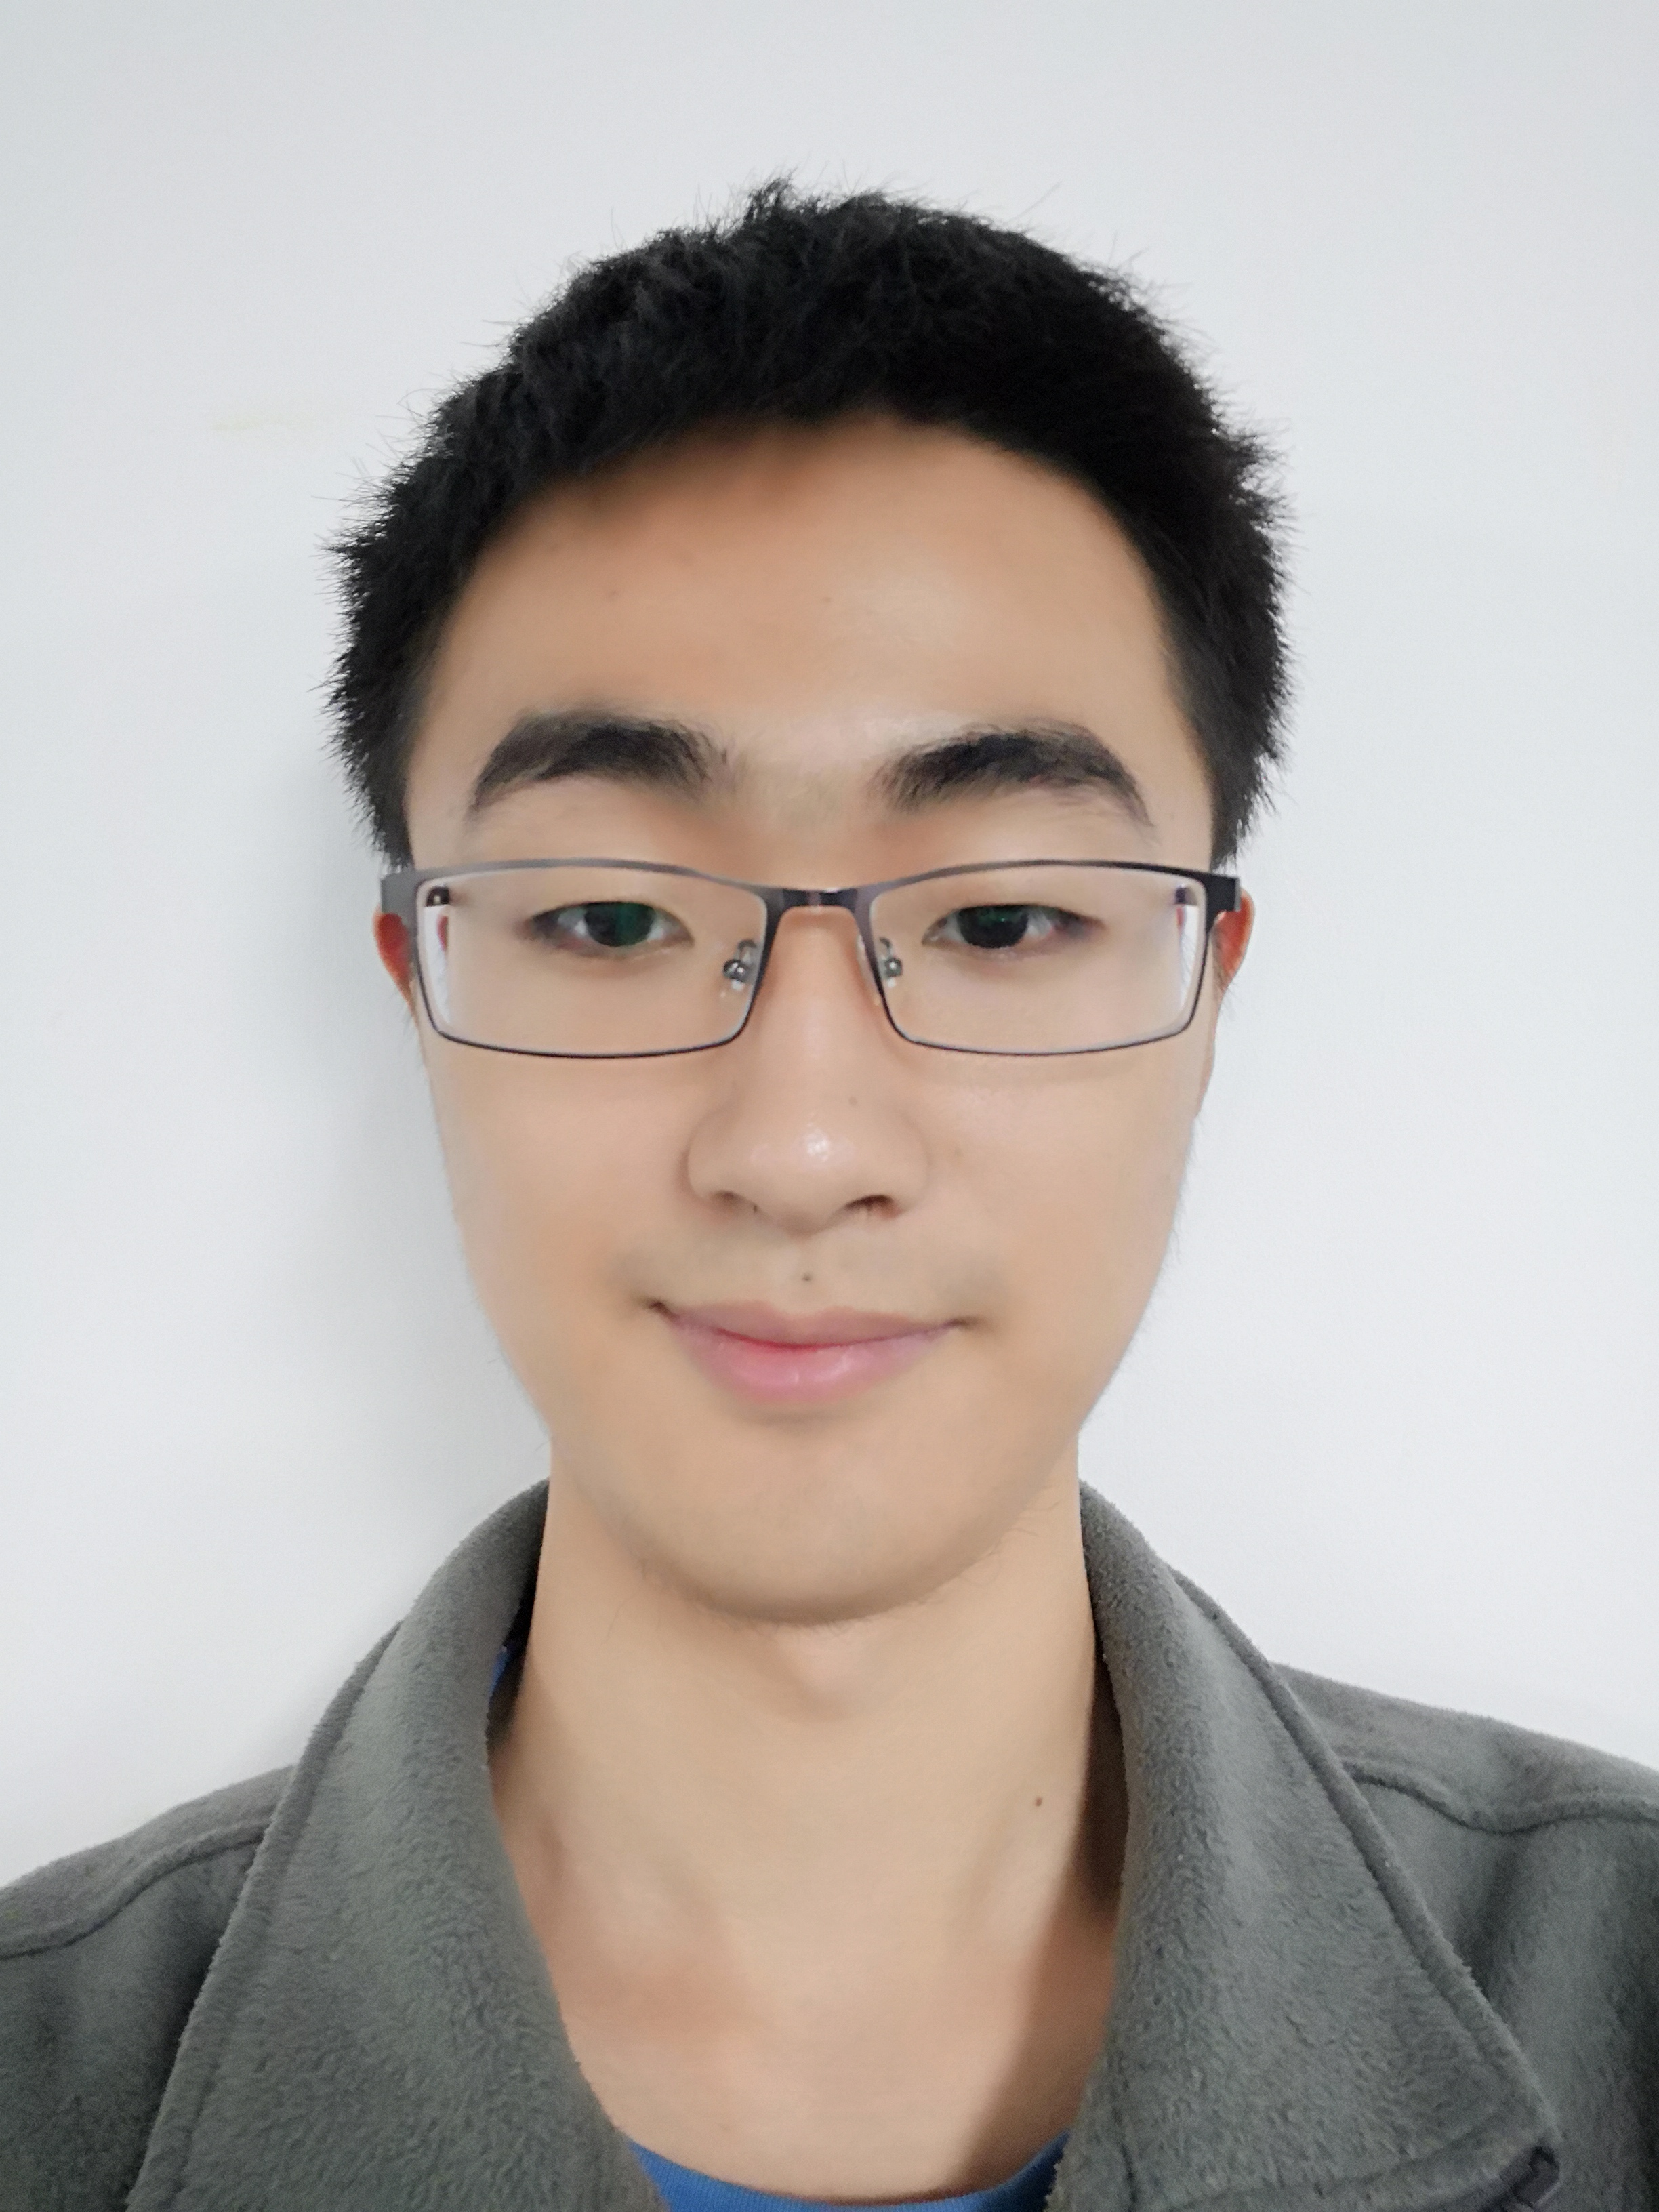
\includegraphics[width=1in,height=1.25in,clip,keepaspectratio]{images/photo/lv.jpg}}]{Bojie Lv}
    (S'18) received the B.E. degree in Communication Engineering from the Southern University of Science and Technology (SUSTech) in 2018, and MPhil degree (ranked top 2) from the Information and Communication Engineering from Harbin Institute of Technology (HIT) in 2020. He is now pursuing the math PhD degree in SUSTech. His research interests are in the area of stochastic optimization and resource allocation in the wireless networks.
\end{IEEEbiography}
\vspace{-1cm}

\begin{IEEEbiography}[{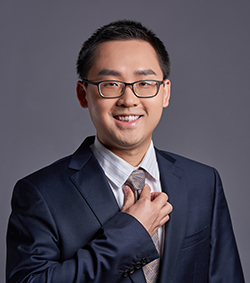
\includegraphics[width=1in,height=1.25in,clip,keepaspectratio]{images/photo/wang.jpg}}]{Rui Wang}
    received the B.S. degree from the University of Science and Technology of China in 2004 and the Ph.D. degree in wireless communications from The Hong Kong University of Science and Technology in 2008.
    From 2009 to 2012, he was a Senior Research Engineer with Huawei Technologies, Co., Ltd. Since 2012, he has been with the Southern University of Science and Technology of China, as an Associate Professor. He has research experience in both academia and industry. He has authored over 30 papers in top-level IEEE journals and flagship international conferences, especially in the area of wireless radio resource optimization and interference management. He has contributed to over 20 U.S. patent applications and over 30 Chinese patent applications (20 of them have been granted). He was also involved in the development of interference mitigation technology for 5G systems.
\end{IEEEbiography}
\vspace{-1cm}

\begin{IEEEbiography}[{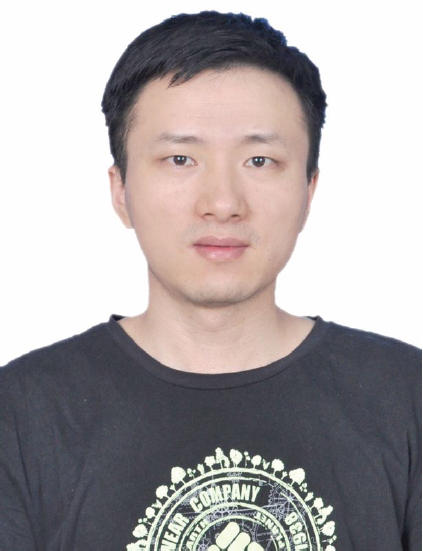
\includegraphics[width=1in,height=1.25in,clip,keepaspectratio]{images/photo/tan.png}}]{Haisheng Tan}
    received his B.E. degree in Software Engineering and B.S. degree in Management both from University of Science and Technology of China (USTC) with the highest honor. Then, he got his Ph.D. degree in computer science at the University of Hong Kong (HKU) in 2011. After that, he worked as a postdoctoral fellow in Prof. Andrew Yao's group at Tsinghua University, Beijing, China. He is currently an associate professor at USTC. His research interests include algorithms and networking. Dr. Tan has published over 50 papers in prestigious journals and conferences, mainly in the areas of wireless networking, data center networks and cloud computing. He recently received the awards of ACM China Rising Star (Hefei Chapter), and the Distinguished Member of INFOCOM 2019 TPC. He is senior member of IEEE.
\end{IEEEbiography}
\vspace{-1cm}

\begin{IEEEbiography}[{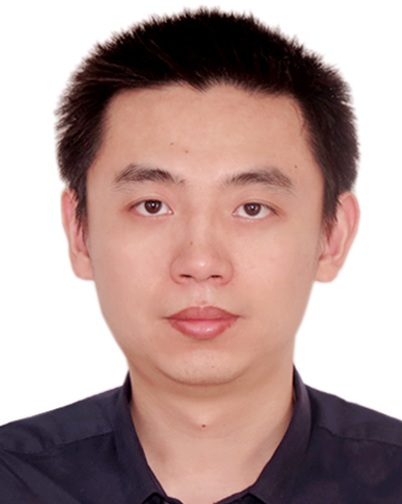
\includegraphics[width=1in,height=1.25in,clip,keepaspectratio]{images/photo/han.jpg}}]{Zhenhua Han}
    received Ph.D. in computer science from the University of Hong Kong, and B.Eng in electronic and information engineering from the University of Electronic Science and Technology of China. He is now a researcher in Microsoft Research Asia. His research interests include cloud computing, AI systems, cluster scheduling. Many of his works have been published in top venues such as USENIX OSDI, IEEE INFOCOM, and IEEE/ACM Transaction on Networking.
\end{IEEEbiography}
\vspace{-1cm}

\begin{IEEEbiography}[{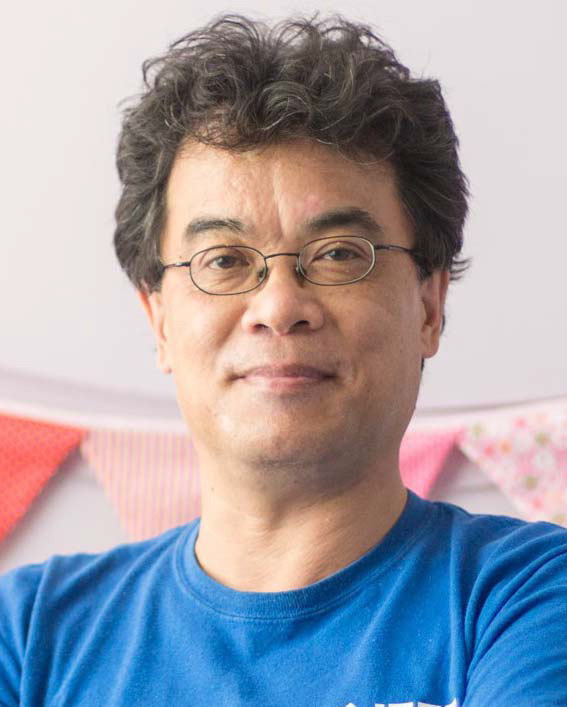
\includegraphics[width=1in,height=1.25in,clip,keepaspectratio]{images/photo/lau.png}}]{Francis~C.M.~Lau}
    received the Ph.D. degree from the Department of Computer Science, University of Waterloo. He is currently an Honorary Professor in and Associate Head (part-time) of the Department of Computer Science at The University of Hong Kong, China. His research interests include computer systems, networks, programming languages, and application of computing in arts. He was the Editor-in-Chief of the Journal of Interconnection Networks from 2011 to 2020.
\end{IEEEbiography}
\vspace{-1cm}
